% Introduction for the Introspective Verification paper.
% Style: plain, direct; no em-dashes; minimal colons/quotes; no anthropomorphic verbs;
% attention to sentence-to-sentence logic. Citation keys are placeholders to be
% resolved against DBLP/CrossRef: processbench (ProcessBench), genprm (GenPRM),
% mathshepherd (Math-Shepherd), azaria2023internal (internal-state probing).

\section{Introduction}
\label{sec:intro}

Reliable multi step reasoning depends on the ability to tell which step first goes wrong, and process reward models supply this signal by scoring each step rather than only the final answer \citep{cobbe2021gsm8k, uesato2022solving, lightman2023lets}. Such scores drive selection and search at test time and shape rewards during training \citep{wang2022selfconsistency, snell2024scaling}. The labels that train these models are costly. They come from human annotation \citep{lightman2023lets}, from Monte Carlo rollouts that estimate whether a step still leads to the correct answer \citep{wang2023mathshepherd}, or from consensus filtering between rollouts and a language model judge \citep{zhang2025lessons}. ProcessBench made step level accuracy directly comparable across methods \citep{zheng2024processbench}, and a recent survey maps the fast growth of the area \citep{zheng2025survey}.

\begin{figure}[t]
  \centering
  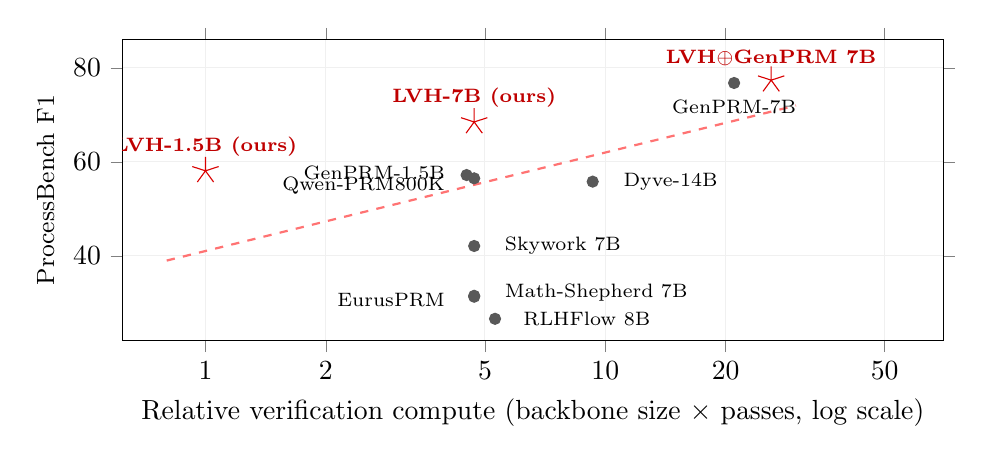
\begin{tikzpicture}
    \begin{axis}[
      width=0.99\linewidth, height=5.4cm,
      xmode=log, log basis x=10,
      xlabel={Relative verification compute (backbone size $\times$ passes, log scale)},
      ylabel={ProcessBench F1}, ylabel style={font=\small},
      xmin=0.62, xmax=70, ymin=22, ymax=86,
      xtick={1,2,5,10,20,50}, xticklabels={1,2,5,10,20,50},
      grid=both, grid style={gray!12}, tick align=outside,
    ]
    % trend guide through the trained baselines
    \addplot[dashed, red!55, thick, forget plot] coordinates {(0.8,39) (30,72)};
    % baseline process reward models
    \addplot[only marks, mark=*, mark size=2pt, gray!70!black, forget plot]
      coordinates {(4.5,57.2) (4.7,56.5) (9.3,55.8) (4.7,42.1) (4.7,31.5) (4.7,31.3) (5.3,26.6) (21,76.8)};
    % ours (three red stars: LVH-1.5B, LVH-7B, and the 7B fusion)
    \addplot[only marks, mark=star, mark size=5pt, red!85!black, forget plot]
      coordinates {(1,58.1) (4.7,68.5) (26,77.4)};
    % our method labels (above the stars, in clear space)
    \node[anchor=south, font=\scriptsize\bfseries, red!75!black] at (axis cs:1,59.0) {LVH-1.5B (ours)};
    \node[anchor=south, font=\scriptsize\bfseries, red!75!black] at (axis cs:4.7,69.6) {LVH-7B (ours)};
    \node[anchor=south, font=\scriptsize\bfseries, red!75!black] at (axis cs:26,78.3) {LVH$\oplus$GenPRM 7B};
    % left cluster: labels extend left into empty space
    \node[anchor=east, font=\scriptsize] at (axis cs:4.2,57.6) {GenPRM-1.5B};
    \node[anchor=east, font=\scriptsize] at (axis cs:4.2,54.9) {Qwen-PRM800K};
    \node[anchor=east, font=\scriptsize] at (axis cs:4.2,30.6) {EurusPRM};
    % right side: labels extend right into empty space
    \node[anchor=west, font=\scriptsize] at (axis cs:10.5,55.8) {Dyve-14B};
    \node[anchor=west, font=\scriptsize] at (axis cs:5.3,42.1) {Skywork 7B};
    \node[anchor=west, font=\scriptsize] at (axis cs:5.3,32.2) {Math-Shepherd 7B};
    \node[anchor=west, font=\scriptsize] at (axis cs:5.9,26.6) {RLHFlow 8B};
    \node[anchor=north, font=\scriptsize] at (axis cs:21,75.3) {GenPRM-7B};
    \end{axis}
  \end{tikzpicture}
  \caption{Introspective verification is compute efficient. Mean ProcessBench localization F1 against the relative compute of one verification, taken as the backbone size times the number of forward passes on a log scale, a rough proxy (the token and wall clock accounting is in \Cref{sec:exp-compute}). The introspective head (stars) sits above the trend of trained process reward models at both scales. From a single forward pass and no generation, LVH-1.5B beats the classification models outright and matches a PRM800K model at 7B and Dyve at 14B, and LVH-7B reaches 68.5 above every same cost baseline. Fused with a generative verifier it passes GenPRM-7B at a small added cost.}
  \label{fig:teaser}
\end{figure}

Two families dominate, and each has a clear limitation. Classification models attach a scalar head to the final layer representation and score a step in one forward pass. They are cheap, but they trail stronger verifiers, in particular on proof heavy problems where the answer is not a single number \citep{zheng2024processbench, zhang2025lessons}, which has motivated label efficient variants that still read from the final layer \citep{yuan2024free, sun2025freeprm}. Generative models close the accuracy gap by writing a critique of each step, and some also generate and run code before a verdict \citep{zhang2024genrm, zhao2025genprm, xiong2025stepwiser, khalifa2025thinkprm}. This accuracy is expensive, because it turns one verdict into a long decoded critique, an interpreter call, and often several samples for majority voting \citep{snell2024scaling}. Adaptive routing lowers the average cost but keeps generation for the hard steps \citep{zhong2025dyve}.

A separate line of evidence points to a cheaper source of the same judgment. A model's hidden states already encode whether its output is correct, which linear probes recover for factual statements and for answer accuracy \citep{azaria2023internal, kadavath2022language, burns2022discovering, marks2023geometry, orgad2024llms, liu2024universal}. Recent work turns these internal signals into rewards for Best of N selection \citep{guo2025mining}, aligns hidden states to improve reinforcement learning \citep{wang2026rightmakesmight}, steers a verifier through its latent representations \citep{zhou2026hidden, hsu2026refine}, and reads step correctness from a frozen backbone \citep{ni2025reprobe}. This evidence has been used mostly for answer level truthfulness, for selection, or for steering. Whether a discriminative read of the hidden states can match a generative process reward model on step level verification, at a fraction of its cost, has not been shown.

We show that this read is possible and competitive. A linear probe on a single intermediate layer of a frozen backbone separates correct from incorrect steps well above chance, and the signal is strongest near seventy percent of the depth rather than at the final layer. We call this operation introspection. The verdict for a step is decoded from the backbone's own intermediate representation, instead of being generated as a critique. This probed signal is stronger at the intermediate layer than at the final layer for a structural reason. The final state is optimized to emit the surface verdict token, so it follows the form of the answer and can be misled by a fluent but wrong step. An earlier state is formed before that token is produced, and it aligns more closely with whether the step follows from its premises. This is a statement about the raw separability of the two layers; once a readout is trained the final layer becomes the stronger single view, and our head combines the two (\Cref{sec:exp-ablation}). The final layer corresponds to what the model would state, while the intermediate layer corresponds to the assessment present before the statement.

Based on this finding, we build an introspective verdict head. The head sums two small readouts, one on an intermediate layer and one on the final layer, and returns a per step reward in a single forward pass. The two readouts and a LoRA adaptation of the backbone are trained on step level correctness labels. Inference uses one forward pass, with no decoding and no code execution, so a solution with $k$ steps is scored at the cost of reading it once. Training fits on a single V100 in a few hours, at the 1.5B scale and at the 7B scale, since a gradient-checkpointed backbone and two small heads stay within one device.

The residual form combines two complementary readouts. Once the backbone is trained, the intermediate layer readout alone is the weaker single view, and the final layer readout alone is strong on easier problems but weaker on proof heavy ones. The sum of the two matches the stronger single readout in mean F1 and improves the proof heavy subsets above either readout alone, so it adds accuracy where accuracy is scarce without giving up accuracy elsewhere.

We evaluate on ProcessBench. With a 1.5B backbone, the introspective head reaches 58.1 mean F1 from a single forward pass (\Cref{fig:teaser}). This exceeds most process reward models evaluated on the benchmark, including trained process reward models such as Math-Shepherd, RLHFlow, Skywork, EurusPRM, and a PRM800K model at 7B to 8B scale, and Dyve at 14B, and it exceeds a generative process reward model of the same 1.5B size. The score approaches the 61.9 of GPT-4o, a much larger general model used as a critic without a process reward model. The cost gap is large. One generative pass of the same size model generates about three times as many tokens as the head reads, so introspection uses about one quarter of the token compute of a single pass, with no autoregressive decoding and no code execution. The two signals are also complementary. A logit space combination of introspection with a generative verifier, with weights fixed on a held out set, improves mean F1 by 5.4 points over the generative verifier alone. At 7B, where the introspective head is again trained on a single V100, the generative verifier is stronger and introspection alone no longer matches it, which marks the regime where generation earns its cost. An unsupervised per domain calibration closes most of the remaining gap, and on 120 case slices the combination raises mean F1 from 76.8 to 77.4 without lowering any subset.

Our contributions are the following.
\begin{itemize}
  \item We identify introspection as a mechanism for process verification. Step correctness is decodable by a probe on the intermediate hidden states of a verifier backbone, where the intermediate layer carries a stronger signal than the final layer.
  \item We build an introspective verdict head, abbreviated LVH, a residual classifier over an intermediate and a final layer that produces per step rewards in one forward pass, trained with LoRA on step labels within a few hours on a single V100, at both the 1.5B and the 7B scale.
  \item On ProcessBench at 1.5B, the head exceeds most trained process reward models on the benchmark, including models at 7B and 14B scale, from a single forward pass that costs about one quarter of one generative pass, and it approaches GPT-4o, which uses no process reward model.
  \item A fixed combination of introspection with a generative verifier improves the generative verifier itself. It adds 5.4 mean F1 at 1.5B, and at 7B, on 120 case slices and with an unsupervised per domain calibration, it raises mean F1 from 76.8 to 77.4 without lowering any subset. We also characterize when introspection is sufficient and when generation is worth its cost.
\end{itemize}

The remaining sections define the head and its training, report the ProcessBench results and the fusion study, and analyze the layer choice and the failure cases.
